
\begin{figure}[h!]
\centering
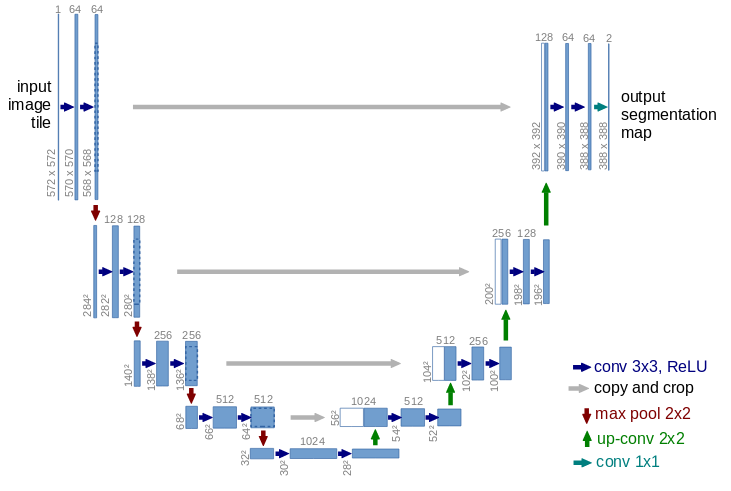
\includegraphics[scale=0.55]{pictures/U-Net}
\caption{The U-Net architecture \cite{uNet}. The left hand side of the U-shape extracts progressively larger features via convolution and pooling. The right side uses these features to produce progressively finer segmentations via upsampling, convolution and concatenation with corresponding feature layers.}
\label{fig:U-Net}
\end{figure}

The U-net architecture is inspired by the success of the FCN architecture, using the technique of concatenating finer layers with coarser ones. Instead of using fractional strides, upsampling is used, where the output is simply the input scaled by an integer $s$ such that a single pixel becomes an $s\times s$ region. Whereas FCN combines all layers at once, U-Net does this layer by layer. After all the convolution and max pooling layers have been applied, the output of the network should then contain the coarsest segmentation. This is upsampled, concatenated with the second coarsest layer, and a convolution is applied. The aim is for this to give a slightly more refined segmentation. This process is continued for each level of coarseness, giving a U-shape to the network (see fig.\ref{fig:U-Net}). In this case the output is not the same size as the input since the finer layers are cropped before being concatenated, but this can be easily changed.